\chapter{Implementation}\label{ch:solution}

\section{System architecture}\label{sec:system-architecture}

The architecture involves three separate MCU units.
The main MCU (\textbf{STM32h747i-disco}) is responsible for the terminal data aggregation and visualization.
Secondary and tertiary MCUs supplement the necessary telemetry.
Sensor modules via the I2C (Inter-Integrated Circuit) bus provide all complex environmental data and to
simulate any immediate interactions, GPIO (General Purpose Input Output) pins are included in the design.
Subsequently, all the communication transfers between the MCUs are secured via the CAN bus that acts as a joint
communication medium.

\begin{figure}[h]
    \centering
    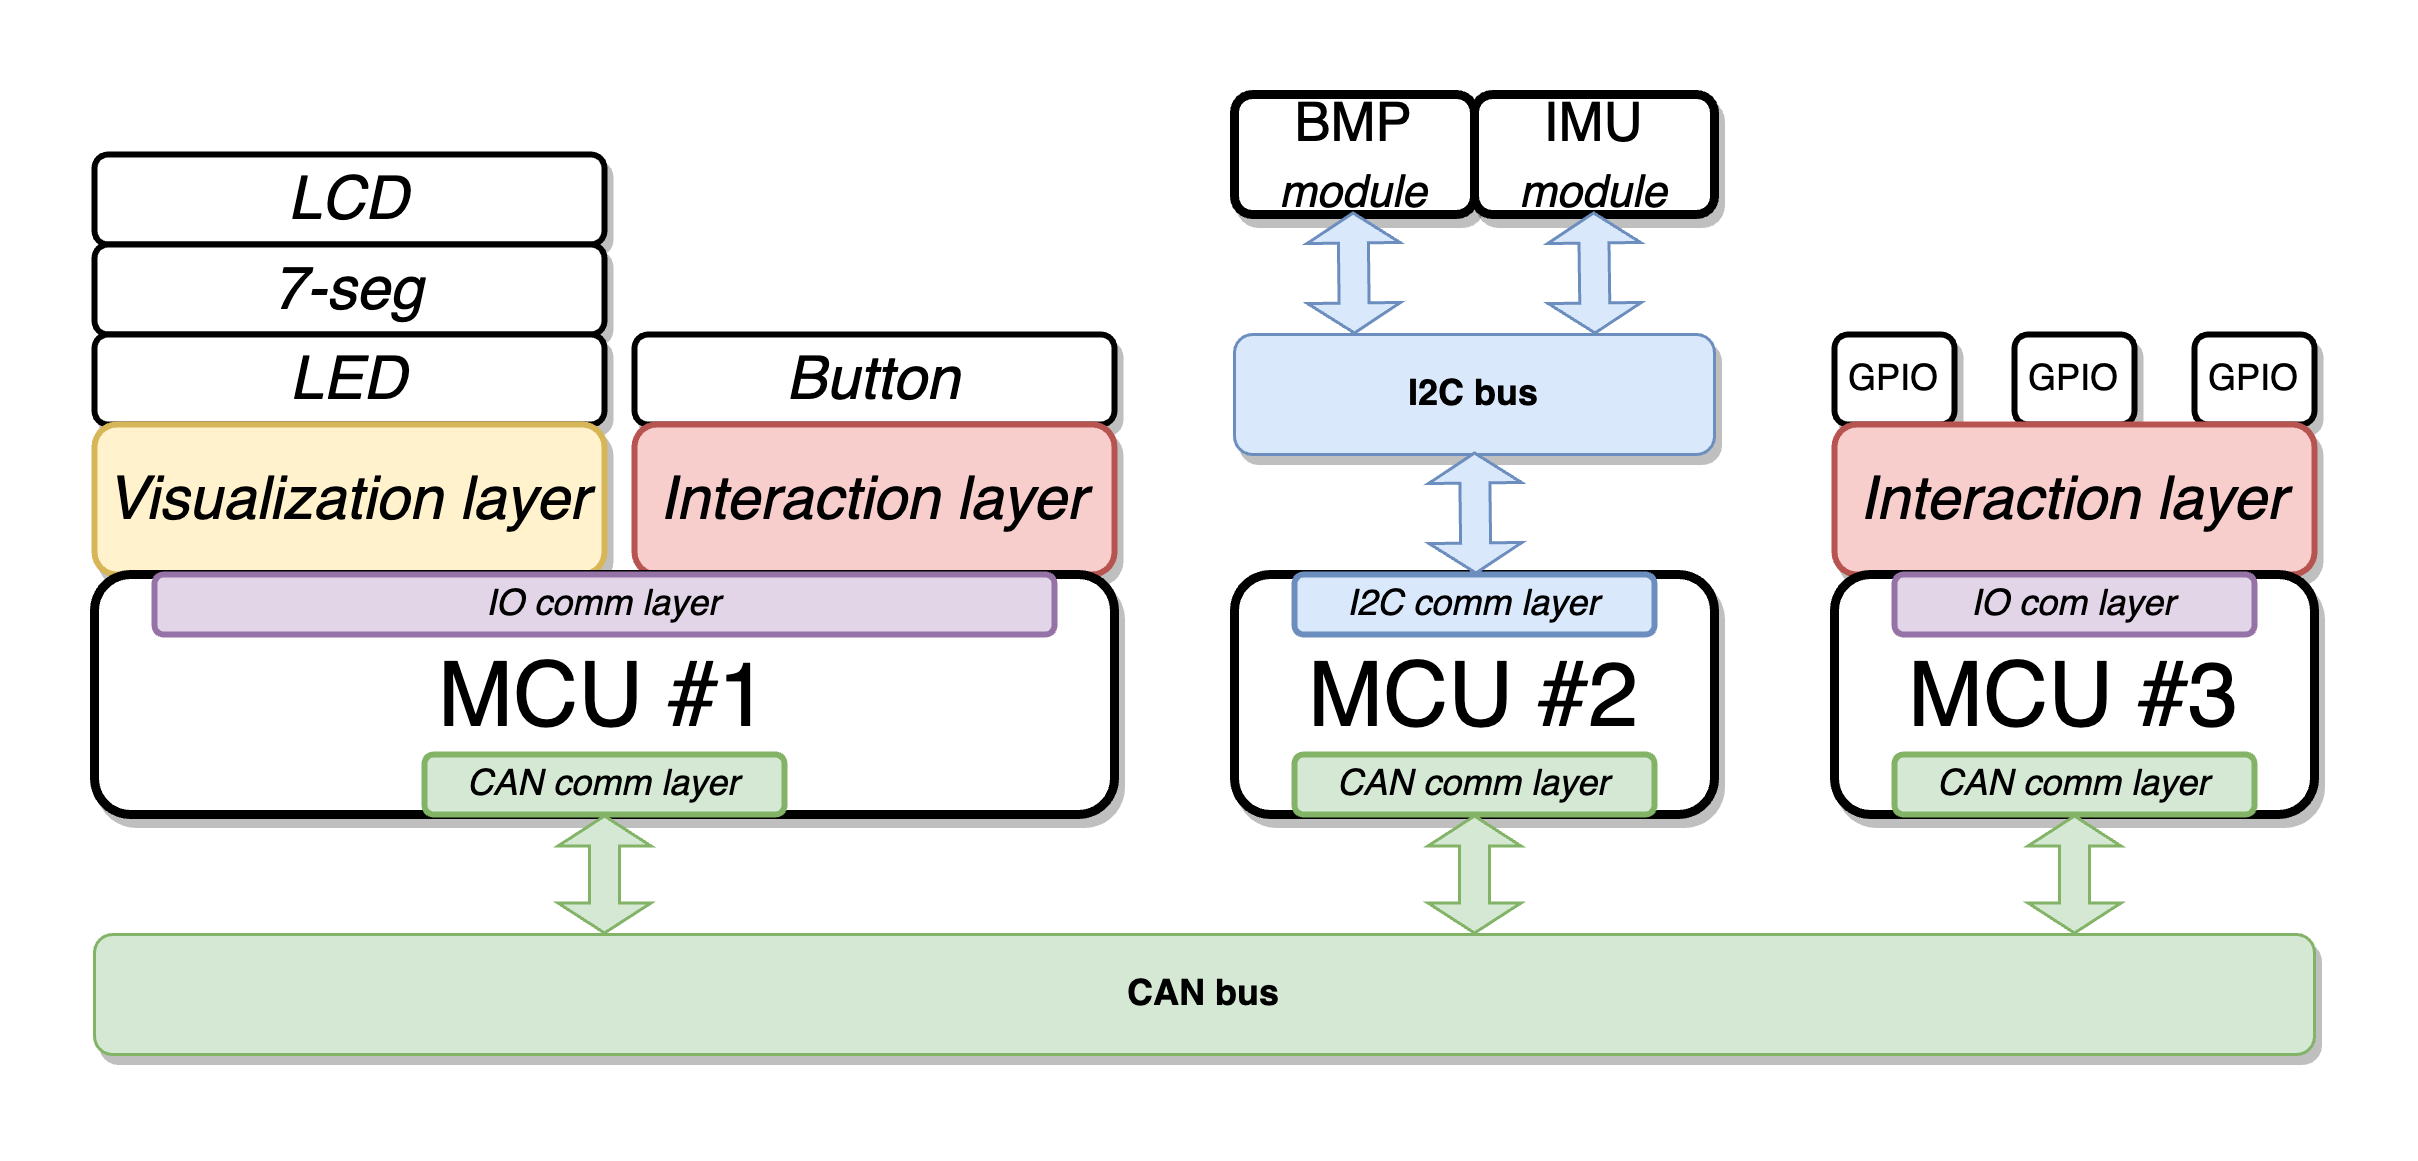
\includegraphics[width=1.0\textwidth]{images/top-level.drawio}
    \caption{Top-level architecture diagram}\label{fig:figure-top-level}
\end{figure}

From the data collection standpoint, the system is designed to acquire telemetry data on both periodic and immediate
basis.
Periodic collection is done by the sensor modules, and an immediate collection is done by the GPIO pins.
This approach allows for a closer representation of the real-world application with various data sources.

\newpage

To furthermore stratify the system, pivotal functionalities are divided into three layers.
\begin{table}[ht]
    \centering
    \begin{tabular}{lll}
        \toprule
        \textbf{Layer} & \textbf{Description} \\
        \midrule
        Communication & Data transfer \\
        \midrule
        Interaction & User inputs \\
        \midrule
        Visualization & Graphical outputs \\
        \bottomrule
    \end{tabular}
    \caption{System functionality layers}
    \label{tab:architecture_layers}
\end{table}

\section{Communication Layer}\label{sec:communication-model}

The communication layer consists of two segments.

\textbf{Primary communication} is done via the CAN bus on a multi-primary (also, multi-master) communication model.
Messages regarding the GPIO data will have the highest priority as they will be
responding to the system's immediate inputs.
Messages with the sensor data will have lower priority and will be sent periodically.
The initial frequency is set to 100Hz. And the CAN bus will be used to encompass all joint communication between the MCUs.

\textbf{Secondary communication} is done via the I2C bus and GPIO pins.
Secondary MCU will use primary-secondary (also, master-slave) communication with the sensor modules through the I2C to
simulate the environmental data.
GPIO pins will be used for simpler digital input signals to simulate immediate interactions.

\begin{figure}[h]
    \centering
    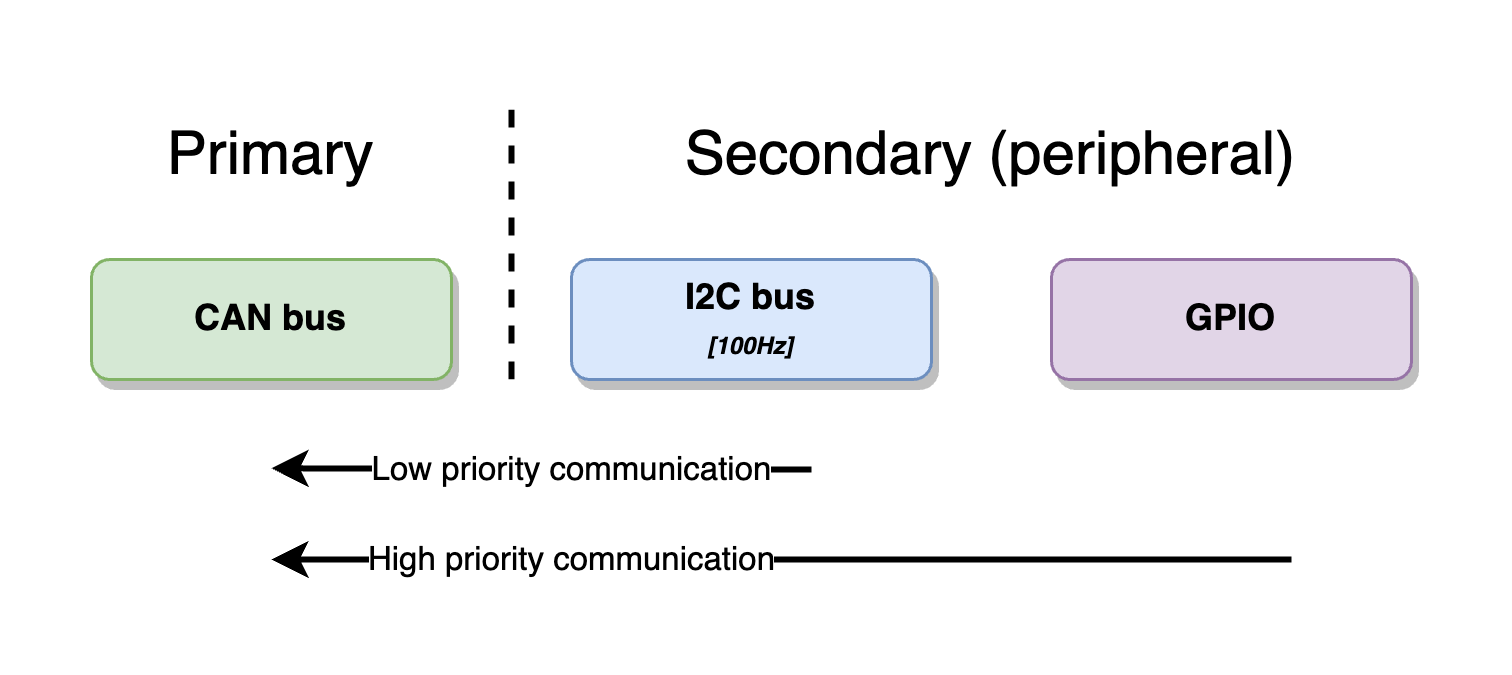
\includegraphics[width=0.8\textwidth]{images/comms.drawio}
    \caption{Communication layer segmentation}\label{fig:figure-comms}
\end{figure}

\newpage

\section{Interaction layer}\label{sec:user-control}

To introduce the element of user control, the interaction layer is divided into two segments.

\textbf{Navigation}, the user can interact with the visualization subsystem via the built-in button.
To switch between different presentation modes and settings.

\textbf{Stimuli}, the user can influence the system's state by providing digital input signals.
By interacting with the GPIO pins, the system should immediately respond and simulate the critical or direct
environmental changes.

\begin{figure}[h]
    \centering
    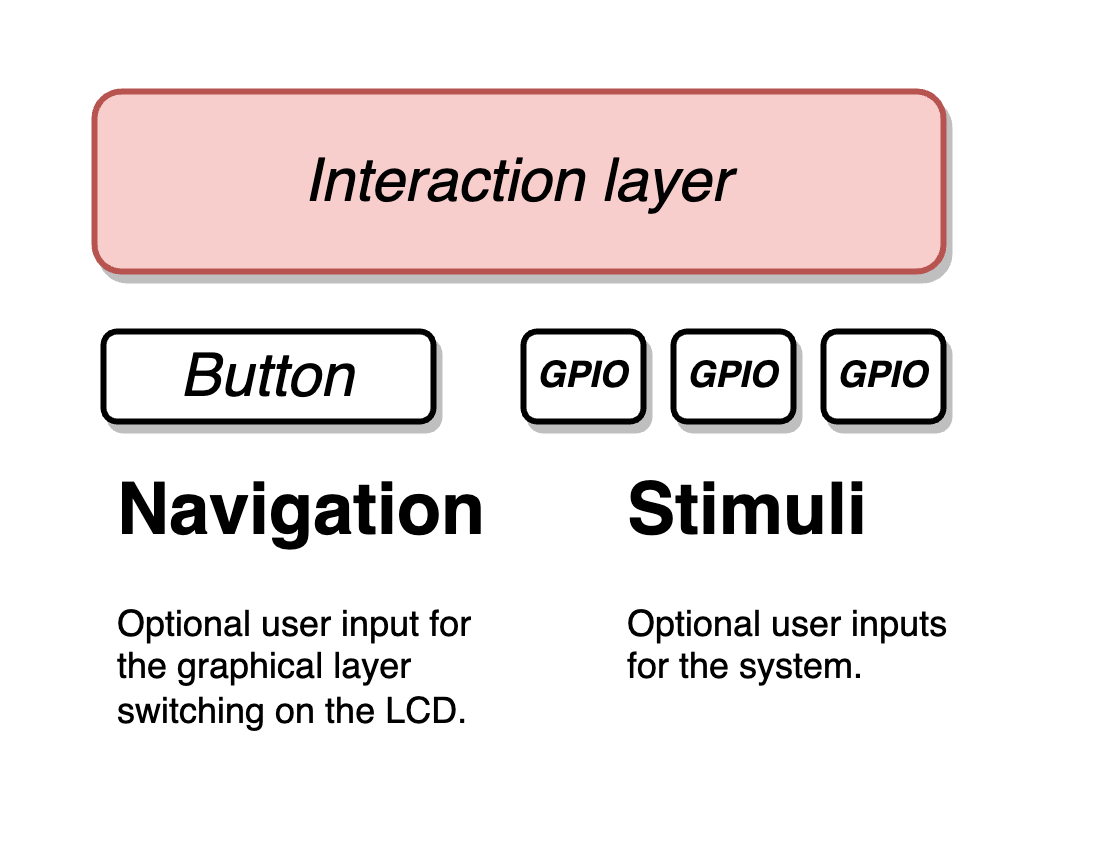
\includegraphics[width=0.5\textwidth]{images/interaction.drawio}
    \caption{Interaction layer segmentation}\label{fig:figure-interaction}
\end{figure}

\section{Visualization layer}\label{sec:gui}

Final visualization is done in three segments.

\textbf{Telemetry}, presentation of the acquired data from the sensor modules.
Concise summary of the measured values with the ability to switch between different data formats and
visualization layers.

\textbf{Navigation}, control cue for the user of the data presentation.
The user is informed about different presentation modes and the current setting.

\textbf{Signaling}, visual feedback of the system's state.

\begin{figure}[h]
    \centering
    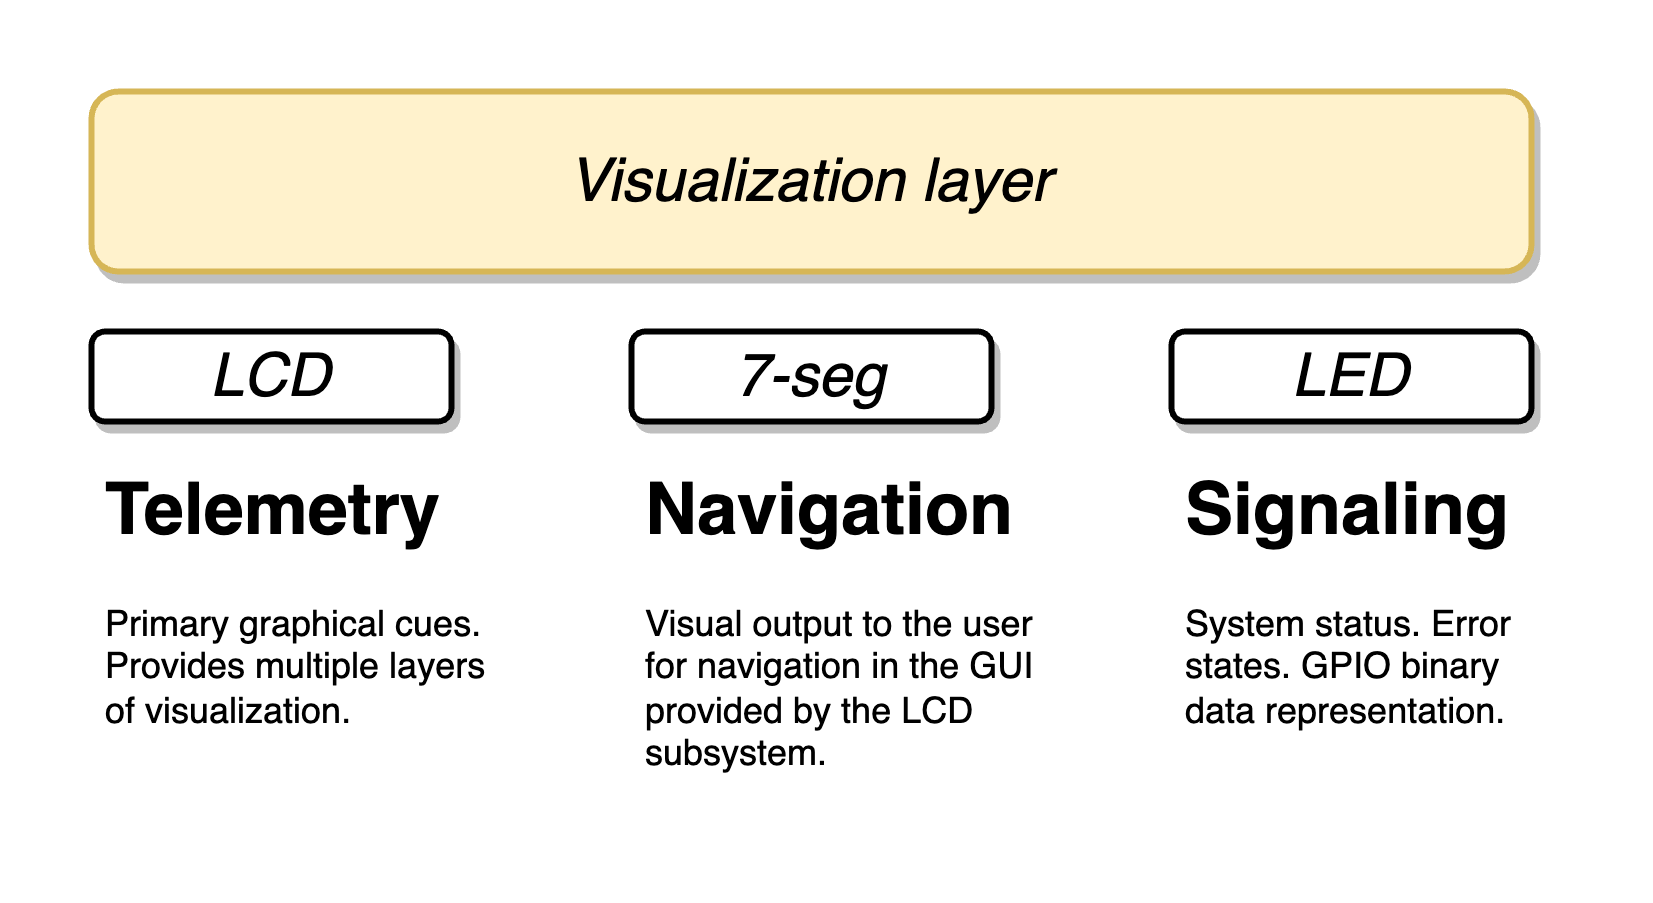
\includegraphics[width=0.7\textwidth]{images/visualization.drawio}
    \caption{Visualization layer segmentation}\label{fig:figure-gui}
\end{figure}
